\chapter{Einleitung}

In der Einleitung wird eine Einführung in das Thema gegeben. Weiterhin werden die wichtigsten Definitionen erläutert und im weiteren die wissenschaftliche Fragestellung, die Ziele und die Arbeitsplanung näher erklärt.

\section{Einführung}

Diese Arbeit behandelt die Neukonzeption des bestehenden Wirbelbettes am Deutschen Zentrum für Luft- und Raumfahrt, Institut für Materialphysik im Weltraum. Ziel ist es das bestehende Wirbelbett zu einem Messaufbau weiterzuentwickeln um Wechselwirkungen in granularen Medien zu charakterisieren. Zur Verifikation der Konstruktion werden im Anschluss Testmessungen mit verschiedenen granularen Medien gemacht. \\
Im Folgenden werden grundlegenden Eigenschaften von Granulaten und Wirbelbetten behandelt. Danach werden die Anforderungen und Ziele erläutert, worauf die Beschreibung der Umsetzung folgt.


\section{Grundlegende Definitionen}

Im weiteren Verlauf wird zunächst erläutert, was granulare Medien physikalisch kennzeichnet und danach das Prinzip eines Wirbelbetts erläutert.

\subsection{Granulare Medien}

Unter Granulat versteht man ein Medium, das aus einzelnen harten Körnern besteht, die jeweils den Gesetzen der Newtonschen Mechanik unterworfen sind. Weiterhin haben die Körner eine Mindestgröße von $\SI{10}{\micro\meter}$, wodurch die thermische Anregung unterbunden wird. \\
Ein weiteres Charakteristikum von Granulaten ist die Dissipation. Das heißt, dass die hauptsächlich kinetische Energie der Körner durch Stöße fast komplett in Wärmeenergie umgewandelt werden kann. \cite{DLRWebsite} \\
Daraus ergibt sich als weiteres Merkmal granularer Medien die Segregation. Das bedeutet, das sich kleinere Partikel zwischen größeren bewegen können und so die Partikel nach Größen aufgetrennt werden. \cite{PhysikimKontext} \\
\hfill \\ 
Wie bei Molekülen gibt es auch bei granularen Medien ein dynamisches Verhalten. Dieses kann man unter anderem hervorrufen, indem man mittels Schwingungen, also Vibration, auf das Granulat einwirkt. Man erhält dann ein schwingungsfluidiertes Granulat, in dem die Bewegung der Teilchen mit der Brownschen Molekularbewegung vergleichbar ist. \\
Die unterschiedlichen dynamischen Zustände des Granulats werden gerne mit den Aggregatzuständen molekularer Stoffe verglichen:


\begin{center}
\begin{figure}[h]
	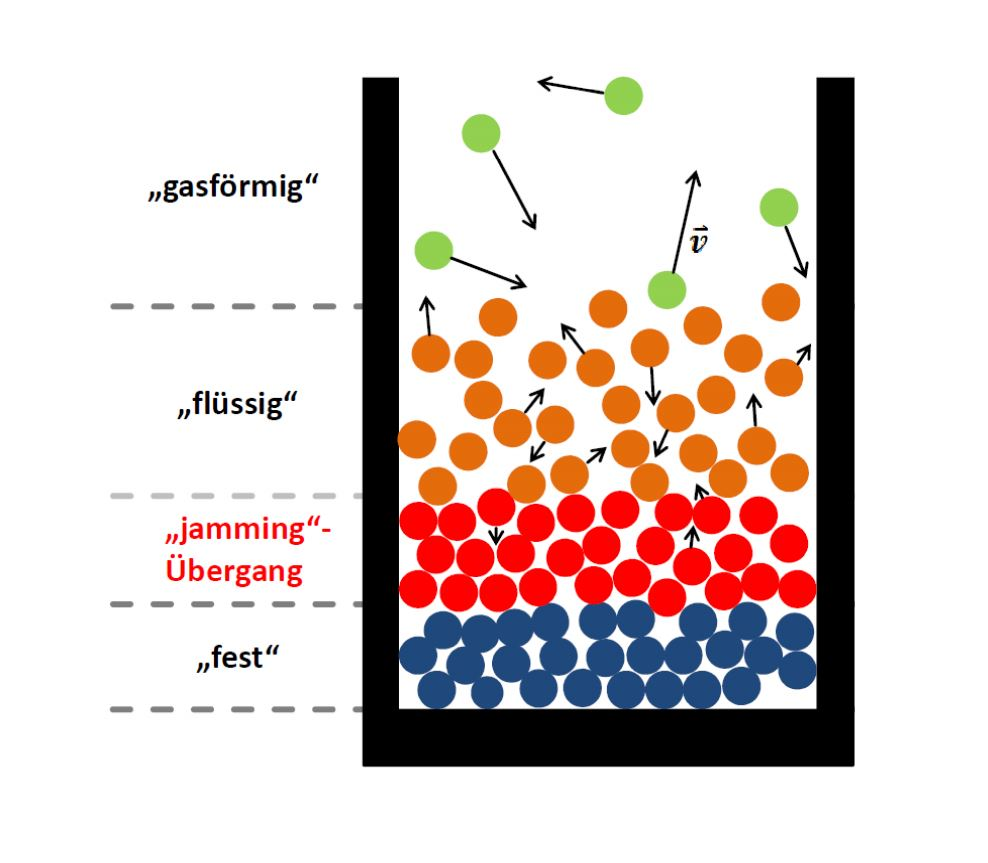
\includegraphics[scale=0.45]{Einleitung_1.jpg}
	\caption[Phasen im Wirbelbett]{Schema eines vertikal vibrationsangeregten Granulatbettes. Man sieht die unterschiedlichen Phasen, die ein Granulat je nach Vibrationsstärke annehmen kann. \cite{Darmstadt2015}}
\end{figure}	
\end{center}

Die in Abbildung 1.1 zu sehenden Phasen treten alle gleichzeitig während einer Anregung durch Vibration auf. Im gasförmigen Zustand sind die Abstände der Partikel weit größer als der Partikeldurchmesser und die Partikel bewegen sich weitgehend unabhängig voneinander. \\
Zum darunter liegenden flüssigen Zustand gibt es, anders als bei Wasser, keinen wohldefinierten Übergang. Man spricht von flüssig, sobald die mittlere freie Weglänge auf die Größenordnung der Partikel gesunken ist. Man spricht auch von einem Glasübergang. \\
Charakteristisch für granulare Medien ist der \glqq jamming\grqq-\ Übergang zwischen fest und flüssig. Hier ist keine Diffusion mehr möglich, die Partikel verbleiben also in ihrer Packungsposition und verklemmen mit ihrer Nachbarn. Bereits in diesem Zustand bilden sich sogenannte \glqq force chains\grqq \ heraus, über die die Kraftübertragung des Systems läuft. \\
Die \glqq force chains\grqq \ bilden sich im festen Zustand vollständig zu einem Netzwerk heraus. Da sich die Partikel amorph anordnen, verlaufen die \glqq force chains\grqq \ nicht homogen und isotrop, sondern willkürlich, was sich in einer unregelmäßigen Kraftverteilung ausdrückt \cite{Darmstadt2015, Fallturmexperiment}.
Eine genaue Charakterisierung der Wechselwirkung in einem granularen Medium mit der Methode von Castellanos möglich \cite{Castellanos2000}. Hierzu wird ein Wirbelbett genutzt, das im folgenden Abschnitt (1.2.2) erläutert wird. Diese Methode macht sich die Eigenschaft zunutze, das sich granulare Medien abhängig von den Wechselwirkungen der Teilchen untereinander und der Größe der Teilchen unterschiedlich verhalten und fluidisiert werden. Fluidisierung heißt in diesem Kontext, dass sich das granulare Medium wie eine Flüssigkeit verhält.

\subsection{Wirbelbett}

Um das Messprinzip von Castellanos zu nutzen und granulare Medien zu fluidisieren, soll folgender Aufbau verwendet werden.


\begin{figure}[h!]
		\begin{center}
		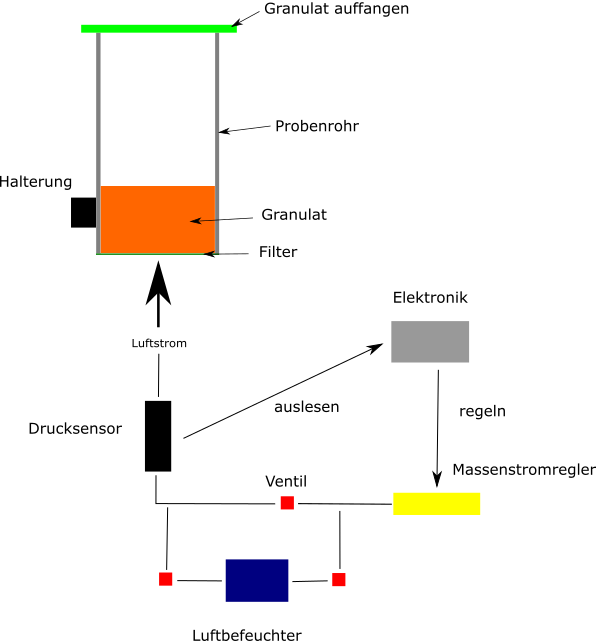
\includegraphics[scale=0.5]{Prinzip_Wirbelbett.png}
		\caption[Messaufbau Wirbelbett]{Schema des Messaufbau zur Charakterisierung von granularen Medien. Luft wird vom Massenstromregler entweder über den Luftbefeuchter oder direkt durch das Granulat geleitet. Dabei wird mit dem Drucksensor der über dem Granulat abfallende Druck gemessen}
	\end{center}
\end{figure}	


Das im Probenrohr befindliche granulare Medium wird von unten von einem durch einen Massenstromregler regelbaren Luftstrom durchströmt. Das Ziel ist hierbei, den Zustand der sogenannten \glqq Fluidisation\grqq \ zu erreichen. Um diesen Zustand messtechnisch zu bestimmen, ist es nötig, den über dem granularen Medium abfallenden Druck sehr genau zu messen. Das Ziel besteht darin, Graphen wie den unten stehenden zu erhalten:

\begin{figure}[h!]
	\begin{center}
		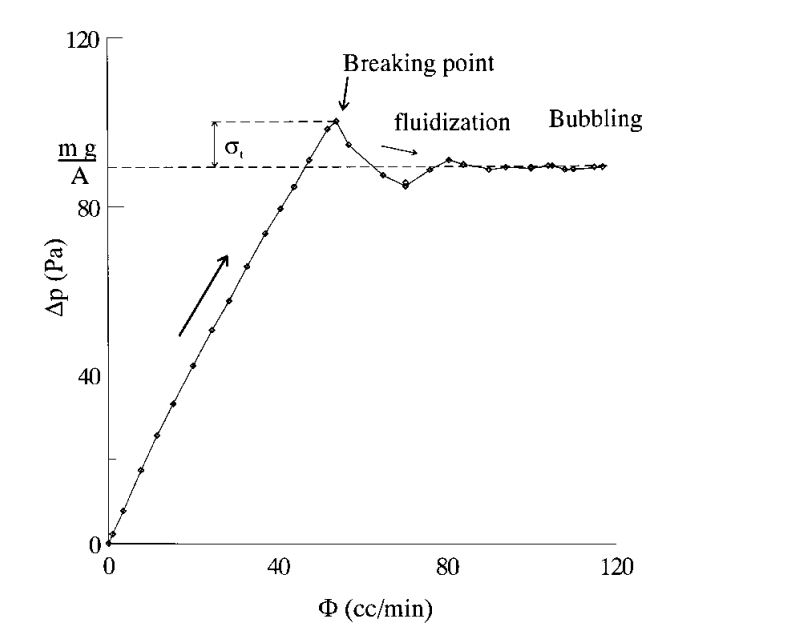
\includegraphics[scale=0.6]{Castellanos_Diagramm.jpg}
		\caption[Fluidisierungsdiagramm]{Druckdifferenz $\Delta p$ (Druck mit Granulat - Druck ohne Granulat) in Abhängigkeit vom Gasstrom. Der Breaking Point ist charakteristisch für das jeweilige Granulat und markiert den Übergang in den flüssigen Zustand \cite{Castellanos2000}}
	\end{center}
\end{figure}

Dabei muss besonders der zu sehende Peak (Breaking Point) gut vermessen sein, da sich über dessen Lage und Höhe die granularen Medien charakterisieren lassen. \\
Neben der Bestimmung mittels Druckabfall, lässt sich der Punkt der Fluidisation auch mittels Lichtstreuung bestimmen. Dazu wird das Ganulat mit einem Laser punktuell bestrahlt. Aus der Änderung des Streulichts lässt sich der Fluidisationspunkt bestimmen. 


\newpage

\section{Derzeitiger Stand und Probleme}


Das bisherige Wirbelbett besteht aus einem eingesteckten Röhrchen mit einem herkömmlichen Schwamm als Filter. Das Röhrchen und die Gaszufuhr sind beide auf einem hohlen Metallblock montiert. Mittels Kleber wird der luftdichte Abschluss erreicht. \\
Das oben beschriebene Teil ist zur vertikalen Verstellbarkeit auf einen Geräteträger montiert, für die horizontale Verstellbarkeit sorgt eine Mikrometerschraube auf dem Geräteträger. 

\begin{figure}[h!]
	\begin{center}
		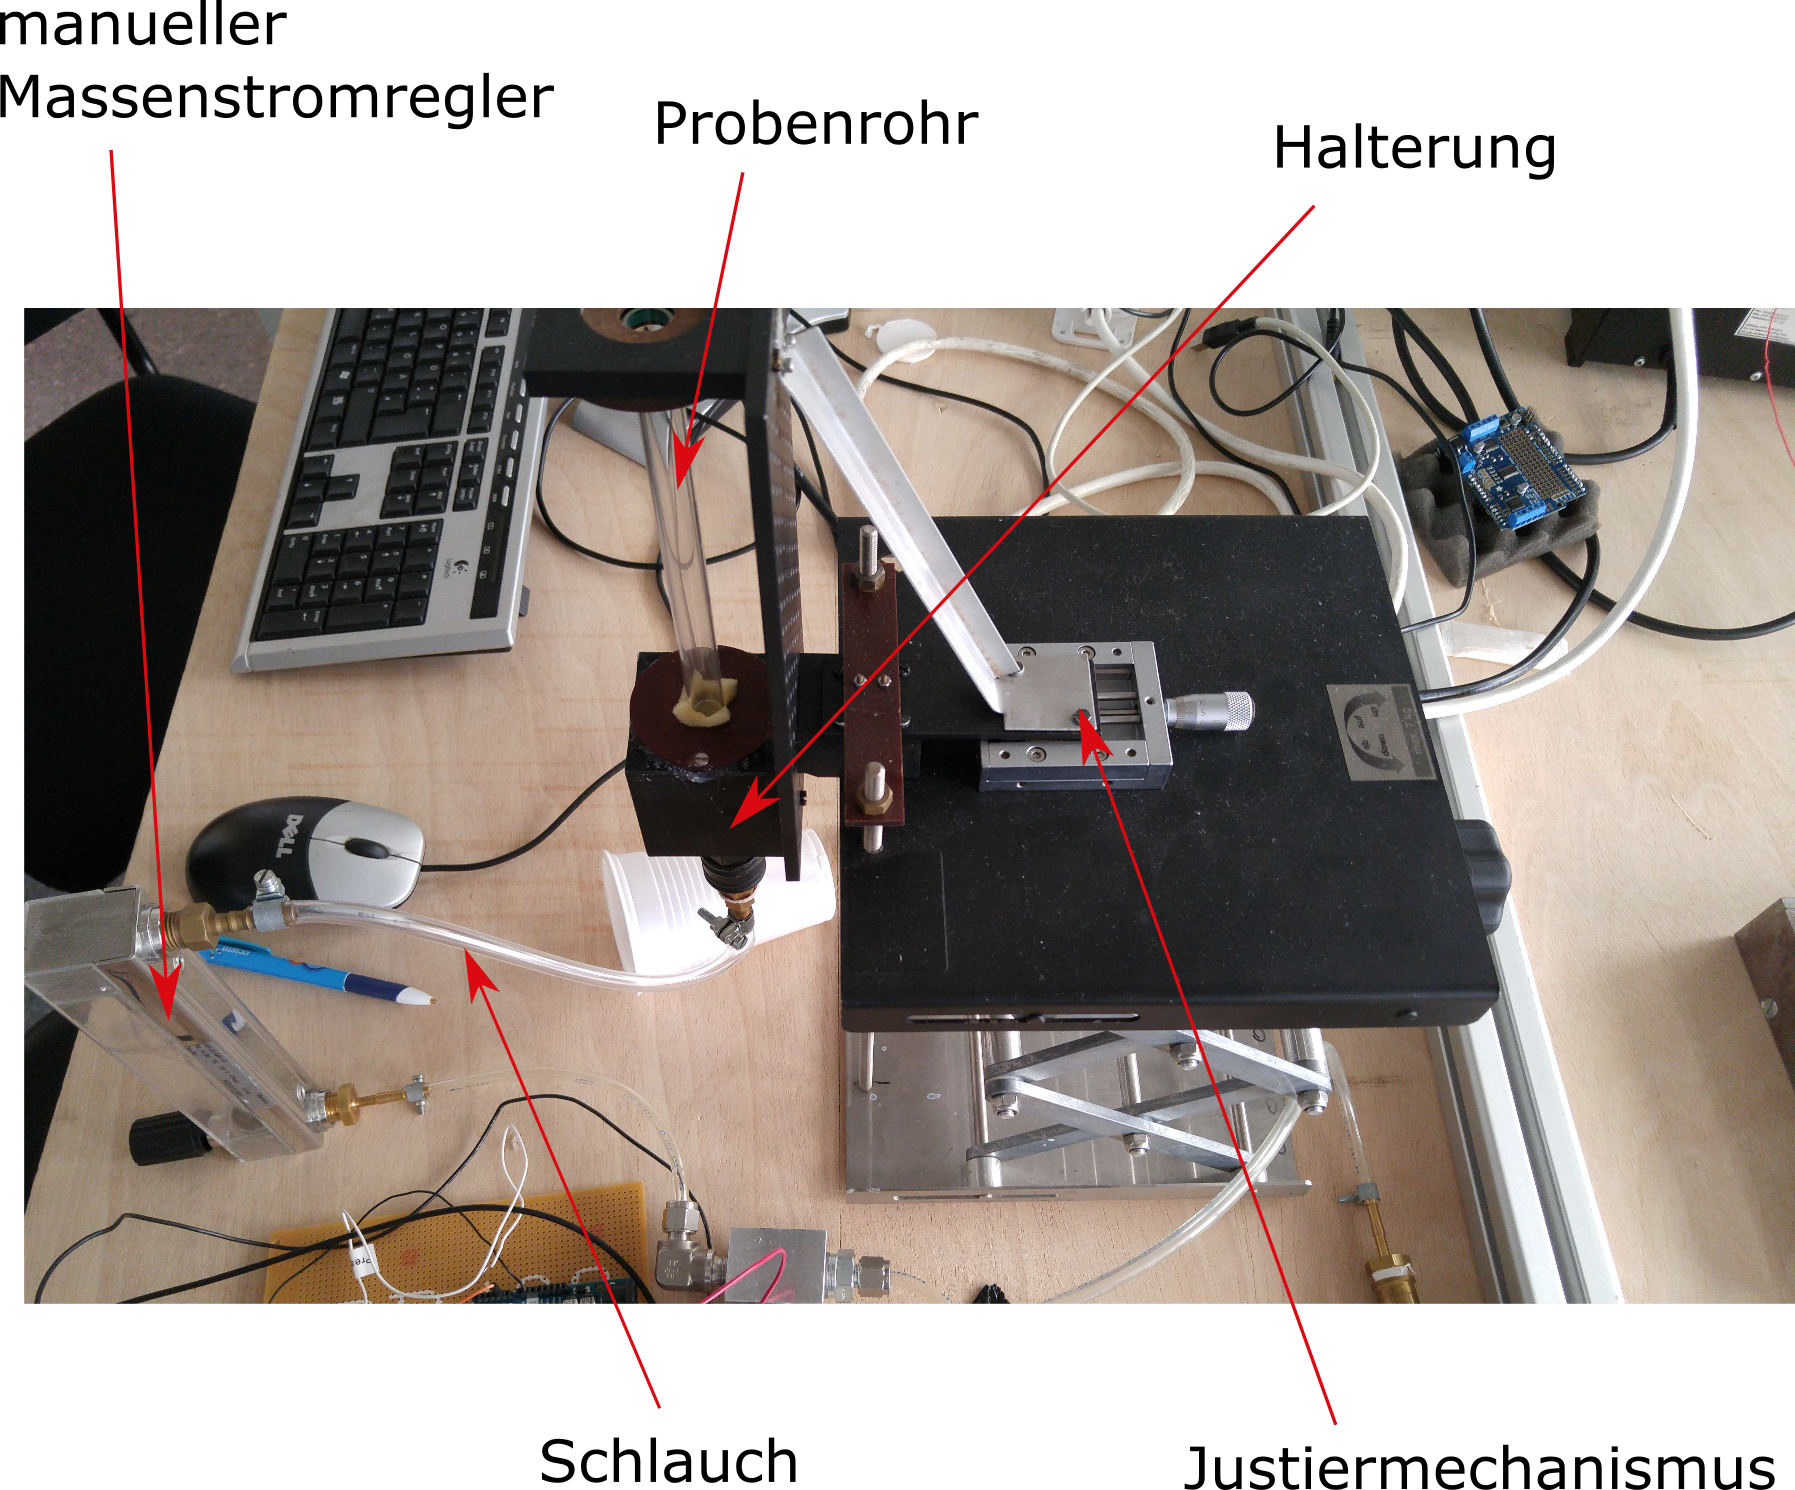
\includegraphics[scale=0.3]{Altes_Wirbelbett_oben.png}
		\caption[Alter Aufbau 1]{Bestehender des Gassystems und der Elektronik.}
	\end{center}
\end{figure}	


Die Gaszufuhr wird über flexible Plasikschläuche realisiert, die teils mit Klemmen und teils mit Muttern an den Geräteflanschen befestigt sind. \\
Die Elektronik zum Auslesen des Drucksensors liegt offen und anfällig auf dem Tisch. Zudem kann der Druck noch nicht genau genug ausgelesen werden. Man bekommt ein Signal zwischen \SIrange{0}{10}{\volt} vom Sensor, das über einen Spannungsteiler auf \SIrange{0}{5}{\volt} reduziert wird. \\
Dieser Aufbau bringt eine Reihe von Problemen mit sich. Das größte Problem ist sicherlich, das nicht mit unterschiedlichen Probenrohrdurchmessern gemessen werden kann. Die sind nötig um auch große Partikel messen zu können. Außerdem ist der luftdichte Anschluss am Probenrohr nicht gegeben, da dies nur mit dem Schwamm in eine Öffnung des Metallblocks gesteckt wird.
Weiterhin ist das Wirbelbett zwar vertikal und horizontal beweglich, aber der Geräteträger verhindert Messungen im Lichtstreuaufbau.
Die bisherige Verrohrung mit Plastikschläuchen ist nicht luftdicht und zu instabil, um reproduzierbar messen zu können. \\


\begin{figure}[h!]
	\begin{center}
		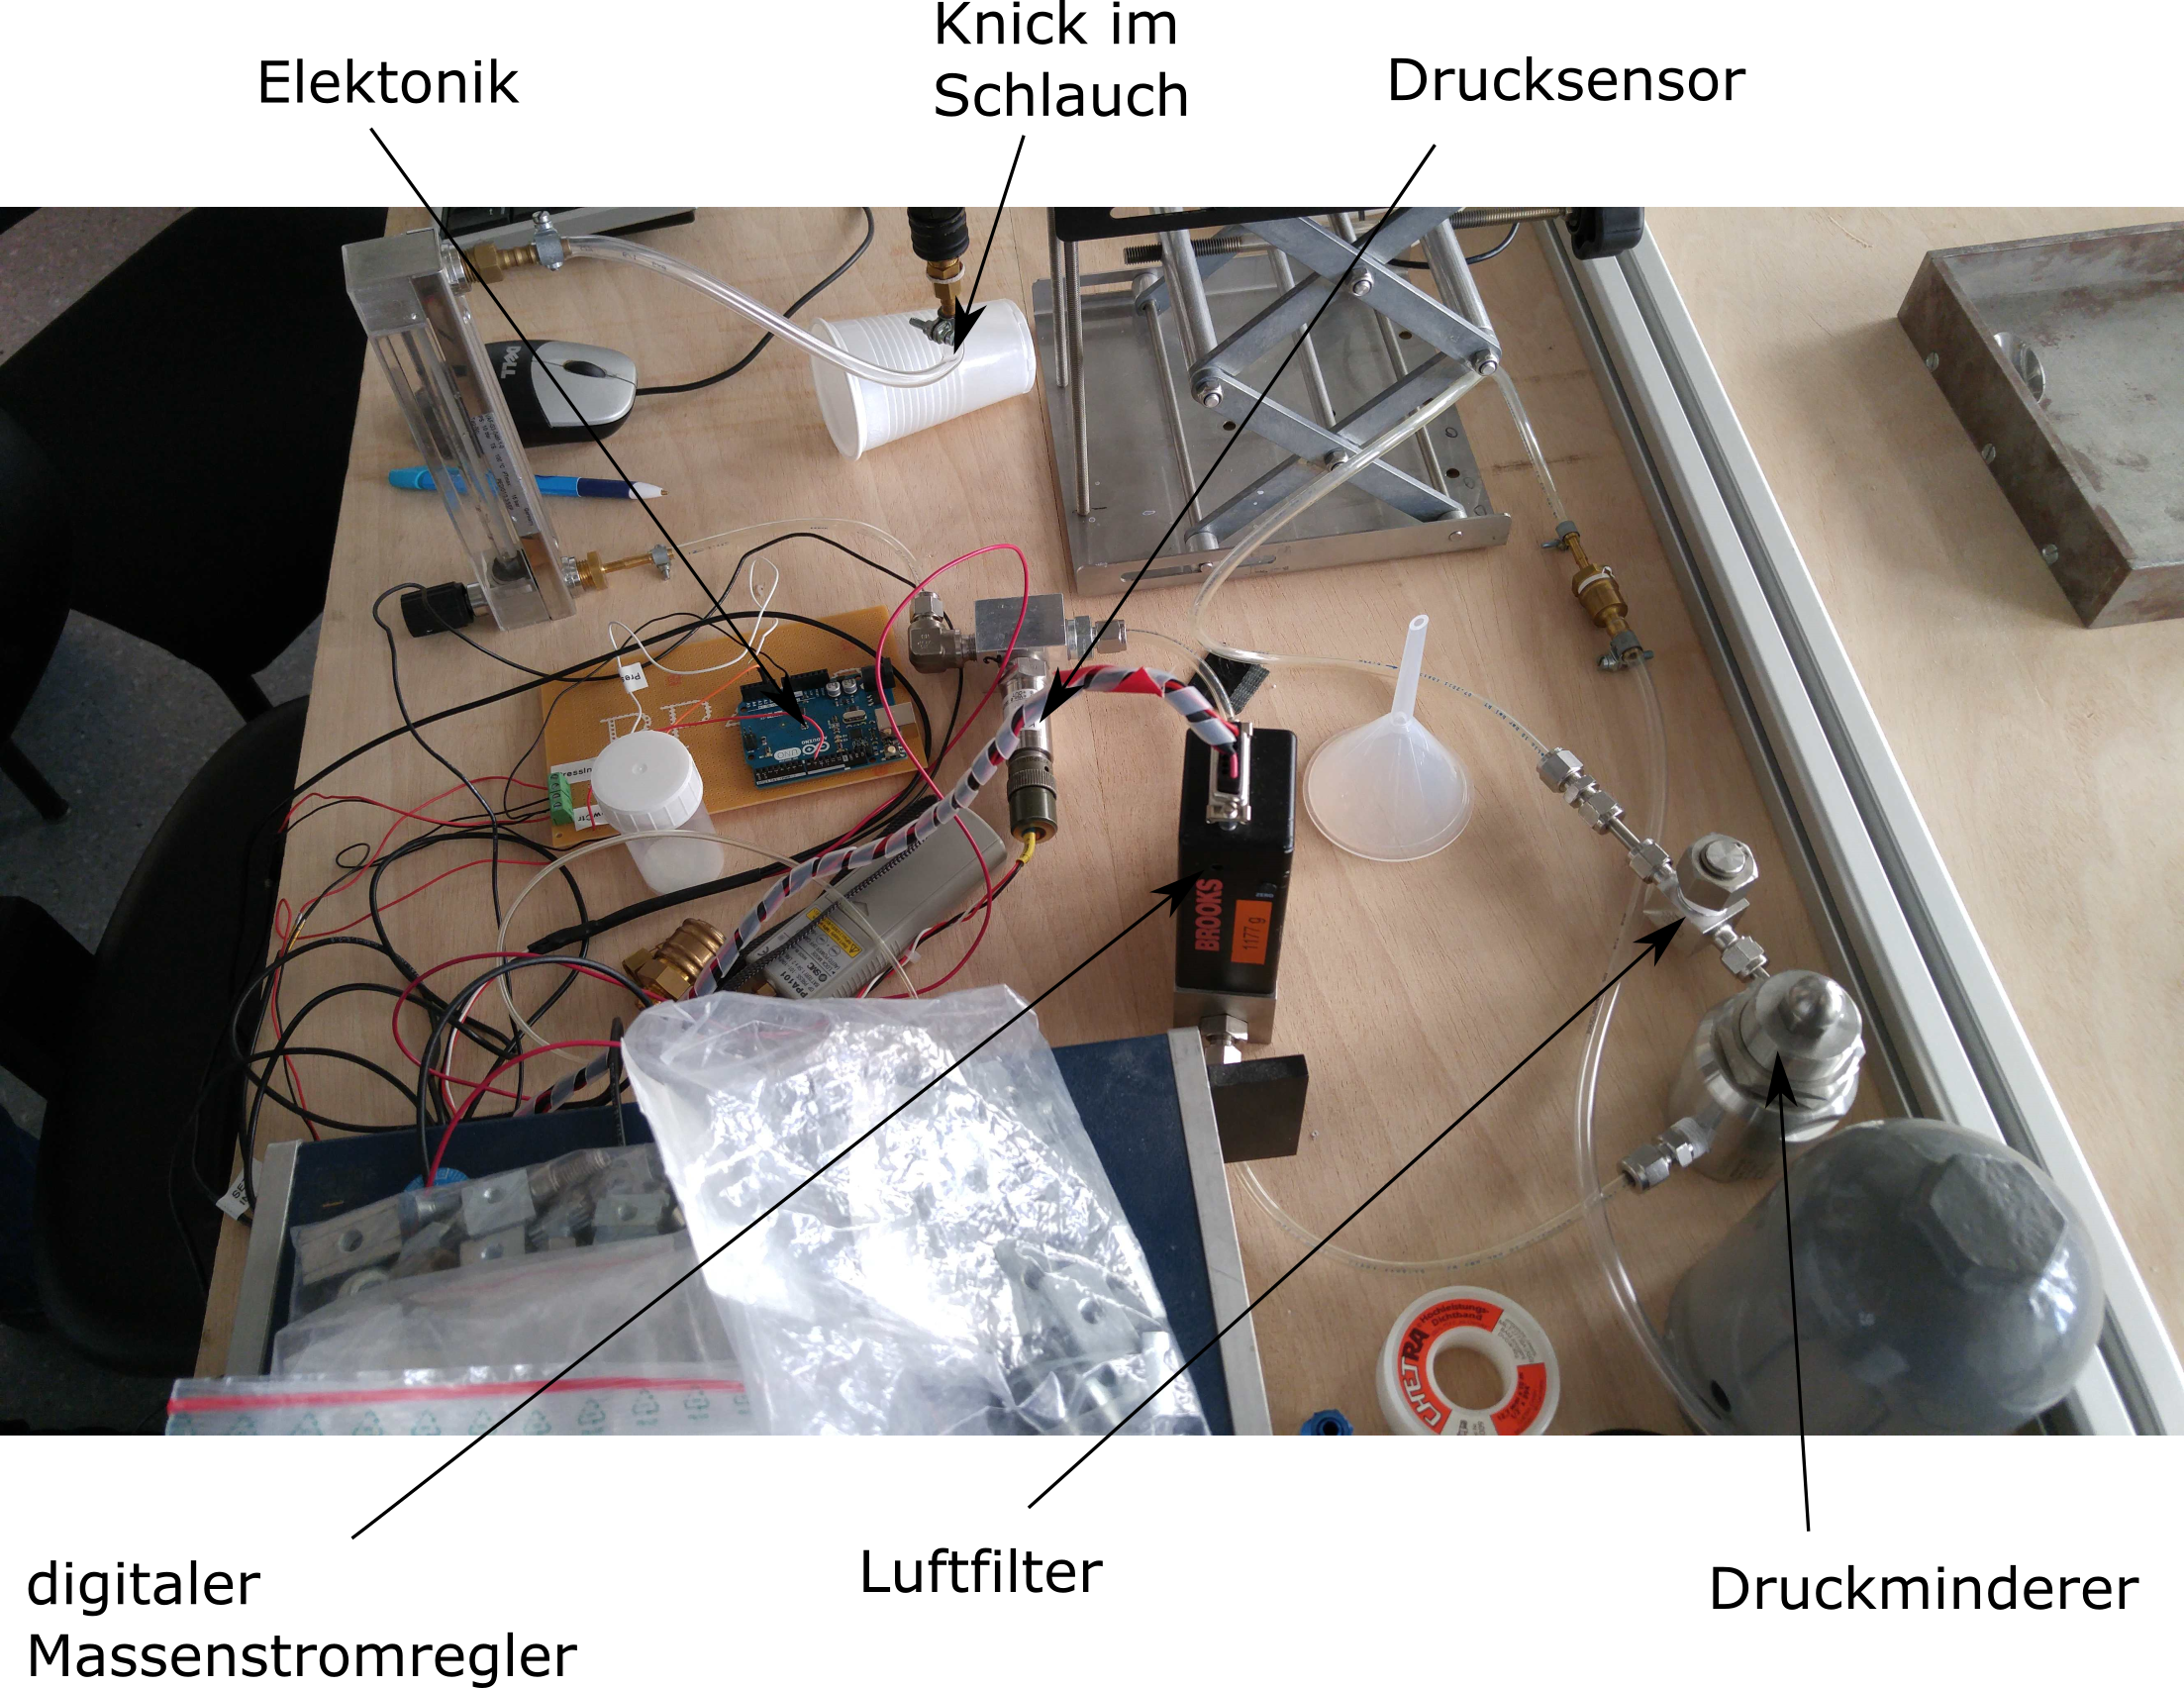
\includegraphics[scale=0.6]{Kabel_Rohrleitungen_alt.png}
		\caption[Alter Aufbau 2]{Bestehende Rohrleitungen und Elektronik}
	\end{center}
\end{figure}


\section{Wissenschaftliche Fragestellung}

Es soll untersucht werden, ob die Wechselwirkung von Partikeln über Beschichtungen kontrolliert werden kann. Die Wechselwirkung soll über den Fluidisierungspunkt mit diesem Aufbau charakterisiert werden. Dazu muss eine große Bandbreite verschiedener Medien quantitaiv messbar sein. In diesem Fall bedeutet quantitativ vor allem, wie schon im vorigen Abschnitt \glqq Wirbelbett\grqq \ beschrieben, sehr hohe Präzision bei der Druckmessung. Dazu braucht man einen luftdichten Versuchsaufbau und einen ausreichend sensiblen Drucksensor. Physikalisch geht es dabei um um folgende Gleichungen: \\
Der Druckabfall über dem Granulat am Punkt der Fluidisation ist mit $\Delta P = \rho h g + \sigma_t$ gegeben. Hierbei ist $\rho$ die Dichte des Granulats und $\sigma_t$ der gemessene Peak aus Abbildung 1.3. Der Druckabfall ist außerdem mit der Carman-Gleichung $\Delta P / h = E \eta U \cdot \frac{1 - \epsilon}{\epsilon^3 d_p^2}$ gegeben. In diesem Fall ist $E$ eine Konstante mit Wert 180, $\eta$ die Gasviskosität, $U$ die Gasgeschwindigkeit, $d_p$ ist der Durchmesser des Probenröhrchens und $\epsilon$ die Porösität des Bettes. \\
Das Ziel der Arbeit ist die Realisierung eines Versuchsaufbau in dem die Strömungsgeschwindigkeit bzw. das Gasvolumen geregelt werden kann und der Druckabfall möglichst präzise vermessen werden kann.


\section{Ziele der Arbeit}

In der vorliegenden Arbeit soll ein vorhandener Versuchsstand für quantitative Messungen weiterentwickelt werden. Zuerst werden die Probleme des bisherigen Setups analysiert und eine entsprechende Lösung für das Medium Luft konstruiert. \\ 
Konkrete Ziele der Bachelorarbeit sind thematisch geordnet folgende:
Die Elektronik soll im Bezug auf das Auslesen des Drucksensors auf \SI{0,1}{mbar} genau sein und in ein Gehäuse verpackt werden. \\
Es soll ein neues Gassystem entworfen werden, das luftdicht und mechnanisch stabil ist. Weiterhin soll in das Gassystem ein Luftbefeuchter integriert werden. Außerdem sollen mit Probenröhrchen mit Durchmessern \SI{5}{mm}, \SI{20}{mm}, \SI{30}{mm} und \SI{40}{mm} gemessen werden. Die Röhrchen sollen einfach und schnell wechselbar sein und auch das Probenmaterial muss einfach zu wechseln sein. Um mit den größeren Röhrchendurchmessern $D_r$ und Partikeln $d_p$ messen zu können muss der Gasstrom erhöht werden. Aus den Gleichungen im vorigen Abschnitt ergeben sich, für die zwei typischsten Packungsdichten ($\epsilon$), folgende Gasströme: 

Gasströme [l/h] für $\epsilon = \SI{0,54}{}$ (zufällige Packung): \\

\begin{center}
	\begin{tabular}{|c|S|S|S|S|}
		\hline
		\diagbox{$D_r$ $[mm]$}{$d_p$ $[\mu m]$}    & 300   & 500   & 750   & 1000 \\
		\hline
		5     & 4,261 & 11,837 & 26,633 & 47,349 \\
		10    & 17,045 & 47,349 & 106,535 & 189,396 \\
		20    & 68,182 & 189,396 & 426,141 & 757,584 \\
		30    & 153,410 & 426,141 & 958,817 & 1704,564 \\
		40    & 272,730 & 757,584 & 1704,564 & 3030,336 \\
		\hline
	\end{tabular}
\end{center}


\vspace{1cm}

Gasströme [l/h] für $\epsilon = \SI{0,64}{}$ (leicht komprimiert): \\

\begin{center}
	\begin{tabular}{|c|S|S|S|S|}
		\hline
		\diagbox{$D_r$ $[mm]$}{$d_p$ $[\mu m]$}    & 300   & 500   & 750   & 1000 \\
		\hline
		5     & 12,831 & 35,643 & 80,197 & 142,573 \\
		10    & 51,326 & 142,573 & 320,789 & 570,292 \\
		20    & 205,305 & 570,292 & 1283,157 & 2281,169 \\
		30    & 461,936 & 1283,157 & 2887,105 &  \textcolor{red}{5132,631} \\
		40    & 821,221 & 2281,169 & \textcolor{red}{5132,631} & \textcolor{red}{9124,678} \\
		\hline
	\end{tabular} 
\end{center}


\vspace{0.5cm}
Aus den Tabellen folgt, das mit einem Gasstrom von \SI{3000}{l/h} fast alle Paarungen abgedeckt werden können. Daher soll der Gasstrom auf diesen Wert erhöht werden. \\
Zur Unterbindung der Elektrostatik des granularen Mediums ist die Integration eines Luftionisators und Luftbefeuchters geplant. Weiterhin soll das Wirbelbett für eine korrekte Integration in den Lichtstreuaufbau horizontal und vertikal manipulierbar sein. \\
Zur Strukturierung der Arbeit wurden die einzelnen Ziele im folgenden Abschnitt unterteilt und ein Zeitplan aufgestellt.

\section{Arbeitsplanung}

Im Folgenden werden die einzelnen Arbeitspakete definiert und ein Überblick auf die zeitliche Einteilung der Abschnitte gegeben. 

\subsection{AP 1 - Analyse}

In diesem Arbeitspaket werden die Eckdaten des Projekts gesammelt und den Anforderungen zugeordnet. Zudem wird über die Materialwahl für das Wirbelbett entschieden und eine Stückliste aller Kaufteile für das Projekt erstellt. Außerdem werden erste Lösungsansätze definiert, was wiederum in die Liste der Kaufteile einfließt.


\subsection{AP 2 - Elektronik}

Aufgabe in diesem Arbeitspaket sind der Bau des Gehäuses und die Erhöhung der Präzision des Drucksensors. Dies soll zu Anfang geschehen, weil die Steuerelektronik für jegliche Steuerung zuständig ist und somit ohne diese das Wirbelbett nicht bedienbar ist. Zudem können mit einem recht einfachen Bauteil wie dem Gehäuse erste Erfahrungen mit dem 3D Drucker gesammelt werden.

\subsection{AP 3 - Gassystem}

Dieses Arbeitspaket beschäftigt sich mit dem Gassystem. Hier geht es insbesondere um das Suchen und Bestellen der geeigneten Teile für die Verrohrung und den Luftbefeuchter, sowie deren Zusammenbau. \\
Der Entschluss, dieses Arbeitspaket auch recht früh anzugehen fiel, auf Grund der langen Lieferzeit für den Flowcontroller. 

\subsection{AP 4 - Wirbelbett}

In diesem Arbeitspaket soll das eigentliche Wirbelbett neu konstruiert werden. Um schnell und effektiv beurteilen zu können, ob die Ideen zielführend sind, soll ein 3D Drucker zur Prototypenerzeugung genutzt werden. Die finalen Teile sollen ebenfalls mit dem 3D Drucker hergestellt werden. \\
Dieser Abschnitt liegt direkt vor dem Testen, damit unmittelbar nach dessen Abschluss alle für den Testlauf nötigen Komponenten vorhanden sind.


\subsection{AP 5 - Tests / Messungen}

Im letzten Abschnitt sollen alle Komponenten im vollständigen Aufbau getestet werden. Hier soll evaluiert werden, ob alle Anforderungen erfüllt wurden und ob es noch Mängel gibt. Kleinere Mängel sollen noch in dieser Phase behoben werden, während bei größeren analysiert werden muss, wie damit umzugehen ist. Wenn möglich werden auch Messkurven des alten Messaufbaus und des neuen verglichen und diskutiert.


\subsection{Zeitplanung}

Graphisch dargestellt stellt sich der Verlauf des Projekts so dar:

\begin{figure}[h]
	\begin{center}
		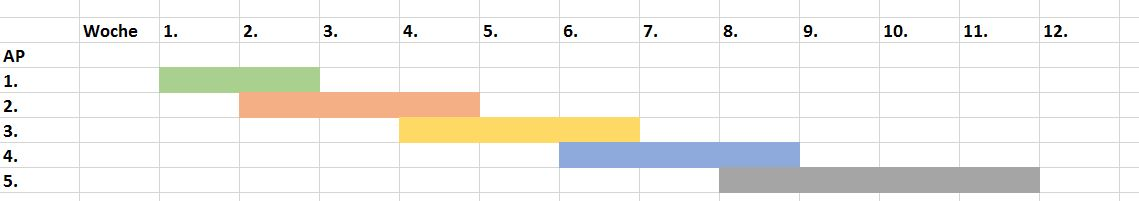
\includegraphics[scale=0.5]{Zeitplan_graphisch.jpg}
		\caption[Arbeitsplan]{Arbeitsplan für die einzelnen Arbeitspakete über die Bearbeitungszeit von 12 Wochen}
	\end{center}
\end{figure}


















